\documentclass[10pt,twocolumn,letterpaper]{article}

\usepackage{iccv}
\usepackage{times}
\usepackage{epsfig}
\usepackage{graphicx}
\usepackage{amsmath}
\usepackage{amssymb}
\usepackage{bbm}

% Include other packages here, before hyperref.

% If you comment hyperref and then uncomment it, you should delete
% egpaper.aux before re-running latex.  (Or just hit 'q' on the first latex
% run, let it finish, and you should be clear).
\usepackage[pagebackref=true,breaklinks=true,letterpaper=true,colorlinks,bookmarks=false]{hyperref}

% \iccvfinalcopy % *** Uncomment this line for the final submission

\def\iccvPaperID{****} % *** Enter the ICCV Paper ID here
\def\httilde{\mbox{\tt\raisebox{-.5ex}{\symbol{126}}}}

% Pages are numbered in submission mode, and unnumbered in camera-ready
%\iccvfinalcopy
\ificcvfinal\pagestyle{empty}\fi
\begin{document}

%%%%%%%%% TITLE
\title{TITLE}

\author{First Author\\
Institution1\\
Institution1 address\\
{\tt\small firstauthor@i1.org}
% For a paper whose authors are all at the same institution,
% omit the following lines up until the closing ``}''.
% Additional authors and addresses can be added with ``\and'',
% just like the second author.
% To save space, use either the email address or home page, not both
\and
Second Author\\
Institution2\\
First line of institution2 address\\
{\tt\small secondauthor@i2.org}
}

\maketitle
\thispagestyle{empty}


%%%%%%%%% ABSTRACT
\begin{abstract}
\iffalse
\noindent In recent years, major advances have been made in 3D scene reconstruction, with a number of approaches now able to yield dense, globally-consistent models at scale. However, much less progress has been made for objects, which can exhibit far fewer unambiguous geometric/texture cues than a full scene, and thus be much harder to track against. Recently, robust, globally-consistent scene reconstruction has been achieved by combining a multi-segment representation with loop closure detection and an online model correction algorithm. The multi-segment approach naturally reduces drift, and the correction algorithm further refines the resulting model. In this paper, we show how to extend this approach to reconstruct accurate, globally-consistent object models. Central to our approach is a novel, probabilistic fusion framework that we use to separate the object of interest from the surrounding scene. We perform both qualitative and quantitative experiments to compare our approach to the current state-of-the-art, and demonstrate compelling improvements in both pose estimation and model quality.
\fi

In recent years, major advances have been made in 3D scene reconstruction, with a number of approaches now able to yield dense, globally-consistent models at scale. However, much less progress has been made for objects, which can exhibit far fewer unambiguous geometric/texture cues than a full scene, and thus be much harder to track against.
In this work we present a novel probabilistic object reconstruction framework that simultaneously allows for online, implicit deformation of the objects surface to reduce tracking drift and handle 
loop closure events. Coupled with our probabilistic formulation is the use of a multi subsegment representation of the object, used to enforce global global consistency, with segmentation of the object 
built in to the formulation. Finally, we employ a CRF framework to refine the overall segmentation, defined by a probability field over the object. We present compelling results over the current state-of-the-art 
object reconstruction work and demonstrate robustness and consistency w.r.t. established dense SLAM frameworks.
\end{abstract}

%%%%%%%%% BODY TEXT
\subsection{Introduction}
Dense Simultaneous Localisation and Mapping (SLAM) has proven very effective for reconstructing moderately-sized scenes,
with much recent research driven by the availability of inexpensive, consumer-grade depth sensing equipment \cite{Newcombe2011,Niessner2013,Prisacariu2014}. 
However, accurate pose estimation in the presence of erroneous measurements and visual aliasing in the scene remains difficult to fully solve. Common approaches \cite{Besl1992,Levoy2001} exploit geometric/texture cues to estimate the pose of each frame, but tracking can drift -- or even fail completely -- without reliable features against which to track.
%Purely geometry based approaches may fail with a lack of descriptive geometry, as may texture based approaches with a lack of texture. 
%Common issues range from tracking drift, often caused by geometric and/or texture ambiguity, to complete tracking failure.
Loop closure events are another common source of tracking problems, with explicit handling often required. Moreover, a failure to handle loop closures correctly can lead to errors in the model, exacerbating any existing tracking issues.
%In addition, many dense SLAM systems fail during loop closure events, with explicit handling often required. The error incurred during loop closure events can be detrimental to tracking quality in such systems.
These problems are only magnified when reconstructing objects: an object's surface will generally contain far fewer points than the full scene, and a lack of unambiguous points on the surface can lead to an increase in data association errors when attempting to recover the pose.

%Failure cases for such approaches are only exacerbated by having less data to track with/against, as is the case with the tracking of an object's pose w.r.t.\ the camera (the inverse of the camera tracking problem). In the case of tracking an object's motion w.r.t.\ the static scene, only the object surface points are available for tracking.

%As dense object reconstruction can be seen as a smaller-scale equivalent of the dense scene reconstruction problem, it too is prone to 
%tracking drift and loop closure issues, sometimes to a prohibitive level. As previously highlighted, the tracking of an object's pose w.r.t.\ the camera 
%is also affected by geometric or texture-based ambiguities, caused by a much more focused domain of the data available to the tracking algorithm. 
%Such failure cases may occur with the presence of ambiguous features, and a lack of unambiguous features on the object surface, causing data 
%association errors when attempting to recover pose.

%For example, when reconstructing an entire scene and assuming no masking, all of the data in the current and previous frames is available for tracking. When tracking solely an object this is not the case as attempting to track an objects movement w.r.t.\ static scene points and dynamic object points would cause a failure event.

Recently, robust, globally-consistent scene reconstruction has been achieved by combining a multi-segment representation with loop closure detection and an online model correction algorithm \cite{Kahler2016}. In this paper, we show how to extend this approach to reconstruct accurate, globally-consistent object models, introducing a probabilistic rigid-object reconstruction framework based on 
depth and texture features. The framework facilitates the correction of tracking drift by representing the object as a
collection of overlapping subsegments between which transformations may be inferred to keep them aligned, resulting in a consistent
overall model. By combining these transformed surfaces, we extract an implicitly deformed surface, optimised for via the probabilistic formulation 
that follows. We utilise a volumetric representation for each of these object subsegments, as with larger-scale reconstruction
systems \cite{Kahler2016}. Each voxel in the subsegments has additional appearance posterior information pertaining to the voxel's membership 
of the object. Over time, multiple volumes containing both surface and probabilistic appearance information are maintained and manipulated to 
yield a robust and temporally consistent model. Finally, we optimise for the optimum object shape within a CRF (Conditional Random Field) framework.

\begin{figure*}[!t]
	\centering
	\begin{tabular}{cccc}
		\fbox{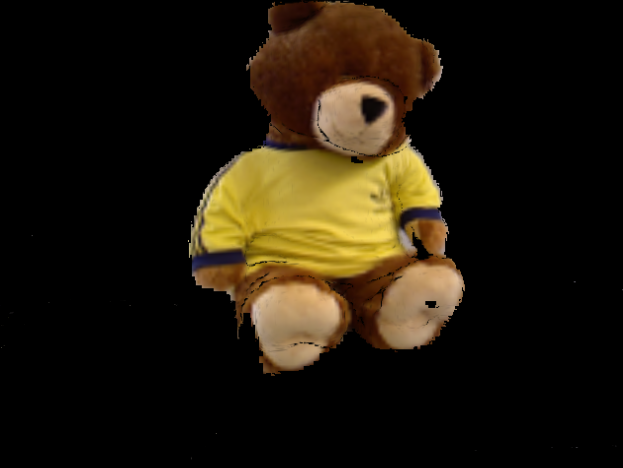
\includegraphics[width=2.5cm]{screenshots/bear_colour.PNG}}&
		\fbox{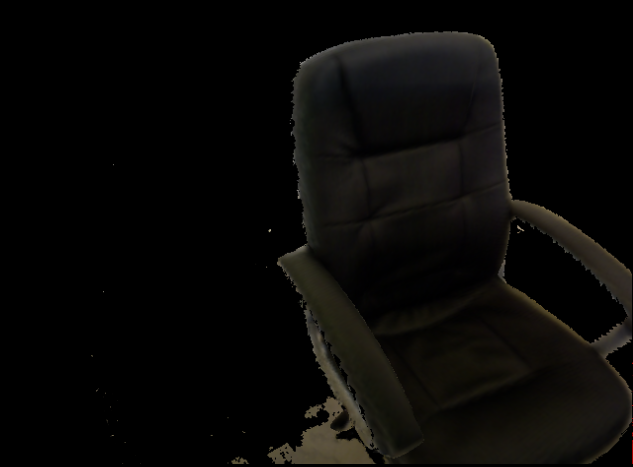
\includegraphics[width=2.5cm]{screenshots/chair_colour.PNG}}&
		\fbox{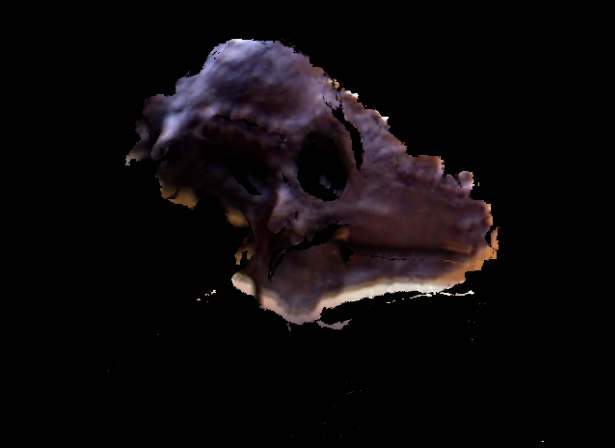
\includegraphics[width=2.5cm]{screenshots/dino_colour.PNG}}&
		\fbox{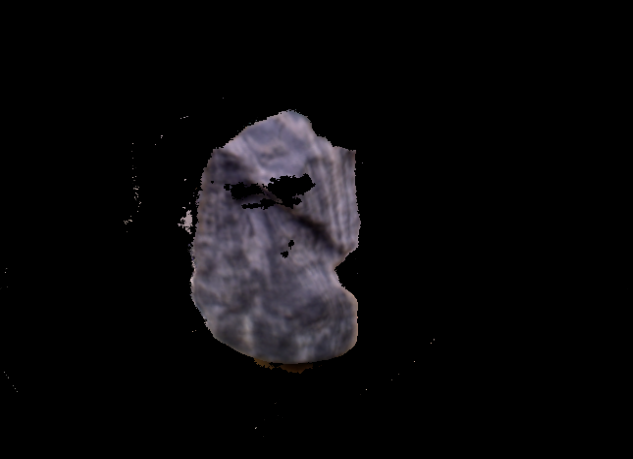
\includegraphics[width=2.5cm]{screenshots/rock_colour.PNG}}\\
		(a)&(b)&(c)&(d)
	\end{tabular}
	\vspace{1mm}
	\caption{
		Reconstruction examples:
		\textbf{(a)} teddy,
		\textbf{(b)} chair,
		\textbf{(c)} dinosaur head,
		\textbf{(d)} rock.
	}
%	\vspace{-5mm}
	\label{fig:demo}
\end{figure*}

%We demonstrate efficacy in object reconstruction by performing online transformations to the aforementioned subsegments to counteract inconsistencies caused by drift in the object pose tracking process.

We perform both quantitative and qualitative experiments to compare our approach to the state-of-the-art object reconstruction approach of Ren et al.\ \cite{Ren2013}, demonstrating compelling improvements in both pose estimation and model quality.

%We perform quantitative and qualitative experiments and demonstrate efficacious pose estimation and reconstruction quality respectively. As a base for comparison, tracking quality is compared with a well established dense SLAM evaluation benchmark \cite{sturm12iros} and reconstruction quality with the object reconstruction system outlined in \cite{Ren2013}.

\iffalse
The motivation behind this work is to improve current semantic scene understanding\cite{Valentin2015, Golodetz2015} by providing a means to procure 
robust object models that can be learnt and recognised. This is a future direction for this and related works.
\fi

%------------------------------------------------------------------------
\section{Background and Pertinent Literature}
\subsection{Dense 3D Reconstruction}
Much 3D reconstruction work in recent years has been influenced by the seminal KinectFusion\cite{Newcombe2011} of Newcombe et al in which
RGBD data was integrated into a volumetric representation of the scene, performing simultaneous tracking and mapping. The end result was
high quality 3D static scene models. 
However KinectFusion notably suffered from tracking drift and had no capacity to handle loop closure
events.

Following KinectFusion, Nie{\ss}ner et al present another volumetric reconstruction system\cite{Niessner2013} based around the notion of
hashing regions of space in to voxel blocks. The primary contribution is the ability to scale the abilities of KinectFusion to larger
scenes. However, the contributions do not extend to the camera tracking drift and loop closure problems.

Prisacariu et al present an alternative voxel hashing based system\cite{Prisacariu2014} which provides many optimisations and an open source 
implementation. However, the limitations of\cite{Newcombe2011,Niessner2013} with regards to loop closure and tracking drift are still present. 
However, a later publication\cite{Kahler2016} from the authors of\cite{Prisacariu2014} presents a loop closure and tracking drift reduction 
solution based on the splitting of the scene in to sub scenes with pose adjustments made to tracking constraints between them, with 
a pose graph optimisation as a final processing step. This approach is extremely pertinent to this work as it inspired the multi subsection approach 
that we take. Dai et al recently introduced a system that improves pose estimation for large scale scenes by considering each previously seen frame within a hierarchical framework and perform sparse feature matching to optimise for the camera pose. However, mismatches between keypoints are reported to have an impact on the robustness of the optimisation procedure.

All of the aforementioned voxel based reconstruction works are closely related to and derived from the early work of Curless et al \cite{Curless1996} 
which introduces the notion of encoding isosurfaces as the zero level of a level set function.

\subsection{Object Reconstruction}
In addition to the larger scale dense SLAM works discussed in the previous section, there has been much work on object reconstruction and 
object-centric SLAM. Ren et al \cite{Ren2013} present a probabilistic object tracking and reconstruction system that, like our work, builds 
object reconstructions based on an appearance model. The presented system evolves a level set object representation for voxels that 
are on the object, as per the appearance model. However, the presented system does not have any provision for loop closure detection and 
is prone to tracking drift over time.

Kolev et al present a probabilistic 3D segmentation and surface extraction algorithm\cite{Kolev2006} based on a variational evolution of a level 
set representation. Object appearance probabilities are fused in to the objects volume for the segmentation, such that the algorithm is robust to 
outliers in the observation images. However, their system does not provide any handling of 
loop closure occurrences and the paper makes no reference to tracking integrity. In addition, the images on which their algorithm was tested 
contained only the objects to be reconstructed, with no background noise.

Another volumetric object reconstruction system is presented by Gupta et al\cite{Gupta2016}, using monocular multi view cues. The authors 
perform object segmentation within a graph cut framework to yield object models and perform tracking based on visual and textual cues. 
However the authors report fluctuating camera tracking quality due to the breakage of brightness constancy and specular surfaces. In addition, 
as with all other works introduced up to this point there is no loop closure ability and tracking drift is an issue.

Slavcheva et al present a volumetric object reconstruction system for RGBD sensors in which pose estimates are yielded by registering pairs of 
SDF(Signed Distance Function) volumes. Unlike many of the aforementioned works, the authors do present a loop closure step, however it is 
performed offline as a post processing step. In addition, the tracking procedure of the presented work is reliant on the use of fiducial markers.

Finally, Weise et al present an explicit, surfel based object reconstruction system\cite{Weise2009} based on objects rotating in front of a 3D 
range scanner. During reconstruction an object topology graph is constructed that is used on-line to handle loop closure cases. When a loop 
closure is detected, if there are discrepancies in the topology graph then deformations are applied locally to patches of the object surface. As 
such, the two misaligned ends of the surface are realigned. In addition, the use of the explicit Surfel based representation makes the reconstructed models less amenable to structured  computation(such as processing by a Convolution Neural Network) than their volumetric counterparts. 

\section{Algorithmic Details}
\subsection{Preliminaries}
\paragraph{Volumetric Representation}
The system we present follows the familiar KinectFusion \cite{Newcombe2011} pipeline for the integration of surface information. In such a 
formulation the scene or object is represented as the zero level of a zero level set \cite{Curless1996}, where the level set is a field of distances 
to the surface and as described, the surface is given by
\begin{equation}
\begin{split}
S = \left\{\psi | \mathcal{D}(\psi) = 0\right\}
\end{split}
\end{equation}
where $S$ is the set of surface voxels, $\psi$ is a voxel in the SDF(Signed Distance Function) volume and $\mathcal{D}(.)$ is the SDF value. 
The SDF volume is truncated to yield a TSDF(Truncated Signed Distance Function) with truncation region $\mu$.

\paragraph{Pose Estimation}
The pose estimation method used in this work is based on the ICP algorithm as used in \cite{Newcombe2011, Prisacariu2014}. The estimation of 
the camera or object 6-DoF pose is formulated as a minimisation problem of the form:
\begin{equation}
\begin{split}
E = \sum_{\omega \in \Omega_{d}} \bigg( \big( R\omega + t - \mathcal{V}(\bar{\omega}) \big) \cdot \mathcal{N}(\bar{\omega}) \bigg)^{2}
\end{split}
\end{equation}
where $\Omega_{d}$ is a depth image, $\omega$ is a 3D point extracted from the depth image, $R$ is an  $\mathbbm{SO}(3)$ 
rotation matrix, $t$ is a translation vector, $\mathcal{V}$ is a rendered depth map from the SDF model, $\mathcal{N}$ is a rendered 
normal map from the SDF model and $\bar{\omega}$ is the point $\omega$ projected into the coordinate frame of $\mathcal{V}$ and 
$\mathcal{N}$.

\paragraph{Surface Integration}
As in previous works \cite{Newcombe2011,Prisacariu2014} we utilise a weighted mean to fuse new depth measurements in to the TSDF model. As such, 
for a new depth measurement $\eta$ projected to by voxel $\psi$, the following update to the TSDF volume $\mathcal{D}$ is made
\begin{equation}
\begin{split}
\mathcal{D}'(\psi) \leftarrow \frac{w(\psi)\mathcal{D}(\psi) + \min(1, \eta/\mu)}{w(\psi) + 1}
\end{split}
\end{equation}
where $w(.)$ is a weighting function and $\mu$ is the aforementioned TSDF truncation region.

\subsection{Representation and Fusion Procedure}
The representation of the object to be reconstructed makes use of multiple `subvolumes' each pertaining to some patch on the object surface. 
New subvolumes are started when a sufficient amount of new voxels have been allocated and have had data integrated. By ensuring overlap 
between the subvolumes, transformations between them can be found. Using the multiple volume approach allows for pose estimation in each 
volume such that pose estimation discrepancies between subvolumes can be detected and are indicative of pose estimation drift.

The proposed system is inspired by\cite{Kolev2006} in that the representation used for the shape of the object to be modelled is a set of volumes 
of probabilities and surface information. The probabilities are posteriors over a per voxel assignment to either the object voxel set or to the non 
object voxel set. In the proposed system this volume of posterior probabilities is built into with each frame, parallel to the fusion process in systems 
such as KinectFusion\cite{Newcombe2011} and InfiniTAM\cite{Prisacariu2014}.

At each frame a probability map is constructed based on the predictions of the model given the current frame. During the fusion process, this 
smaller volume is mapped into as a source of voxel wise appearance probability information. The overall appearance based posterior for a given voxel 
$\psi \in \Psi$ takes the following form:
\begin{equation}
\begin{split}
P(\psi \in \Phi | \Omega, p) = \prod_{t=0}^{\infty} P(\psi_{t} \in \Phi_{t} | \Omega_{t}, p_{t})
\end{split}
\end{equation}
where $\Psi$ is the volume of voxels for which measurements are accumulated, $\Phi$ 
is the volume of voxels pertaining to the object, $\Omega_{t}$ is the current image observation at time $t$ and $p_{t}$ is the 
currently tracked pose at time $t$.
The above encodes the probability of a voxel belonging to an object as the product of the instantaneous conditionals for observations at each time step. 
Note that in general $\Phi \subset \Psi$, and the use of $\Phi$ in the above equation is an abuse of notation as in the above 
$\Phi$ is a discretisation of the continuous $\Phi$ in the probabilistic formulation that follows. Finally, note that a conditional 
independence assumption is made to aid computational tractability in the model.

\subsection{Probabilistic Formulation of Object Reconstruction}
As previously highlighted, central to the proposed system is a volume of posterior probabilities pertaining to a voxel wise membership of either the 
object set or the non object set. This allows one to formulate the full joint distribution over the object as the Probabilistic 
Graphical Model of Figure \ref{pgm1}.
\begin{figure}[!t]
	\centering
	\subfigure[]{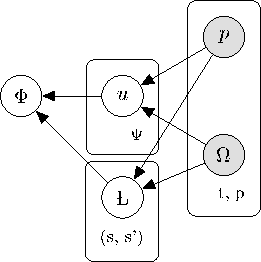
\includegraphics{graphical_models/pgm1.pdf}\label{pgm1}}%
	\hspace{12mm}%
	\subfigure[]{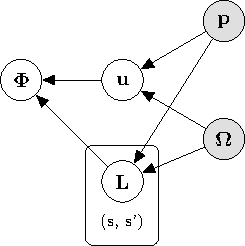
\includegraphics{graphical_models/pgm2.pdf}\label{pgm2}}
	\caption{(a) An initial probabilistic formulation of the object reconstruction pipeline, and (b) a simpler formulation based on various simplifying assumptions (see text).}
\end{figure}

Where $\Phi$ is the shape to be reconstructed, $u$ is the appearance model volume, $L$ is the 
set of consistency constraints for each adjacent sub volume pair in the form of rigid transformations, $\Omega$ is the set of 
RGBD image pixels and $p$ the set of poses over time.

This gives rise to the following analytical formulation of the above distribution:

\begin{equation}
\begin{split}
P(\Phi, \Omega, p, u, L) = 
\prod_{\psi \in \Psi}\prod_{(s, s') \in \mathcal{S}}P(\Phi|u_{v}, L_{(s, s')}) 
\prod_{t=0}^{\infty}\prod_{p \in \mathcal{P}}\\
P(u_{v}|\Omega_{p, t}, p_{t})
P(L_{(s, s')}|\Omega_{p, t}, p_{t})
P(L_{(s, s')})P(p_{t})P(\Omega_{p, t})
\end{split}
\end{equation}
where $\mathcal{V}$ is the set of voxels across all sub volumes, $\mathcal{P}$ is the set of RGBD pixels for a given 
frame and $\mathcal{S}$ is the set of sub volumes.

However, if one were to assume temporal and pixel wise independence in the RGBD observations and temporal independence in 
the poses, the plate containing $\Omega$ and $p$ can be removed:
\begin{equation}
\begin{split}
P(\Phi, \Omega, p, u, L) = 
\prod_{v \in \mathcal{V}}P(\Phi|u_{v})
\prod_{(s, s') \in \mathcal{S}}P(u_{v}|\Omega, p, L_{(s, s')})
P(L_{(s, s')}|\Omega, p) P(L_{(s, s')})P(p)P(\Omega)
\end{split}
\end{equation}
In practice this temporal independence assumption causes no issues.

Furthermore, if one assumes voxel wise independence, the plate over voxels can be removed. Finally, assuming $P(p)$ and 
$P(\Omega)$ are uniform distributions, then we have the simpler distribution given by Figure \ref{pgm2}.

\iffalse
\begin{figure}[!t]
	\centering
	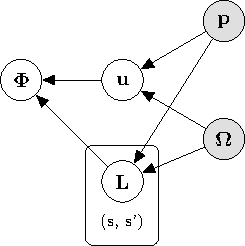
\includegraphics{graphical_models/pgm2.pdf}
	\caption{Simplified probabilistic formulation of the object reconstruction pipeline.}
	\label{pgm2}
\end{figure}
\fi

Where the simpler distribution takes the following analytical form:
\begin{equation}
\begin{split}
P(\Phi, \Omega, p, u, L) = 
\prod_{(s, s') \in \mathcal{S}} P(\Phi|u, L_{(s, s')})
P(u|\Omega, p)
P(L_{(s, s')}|\Omega, p)
P(L_{(s, s')})
\end{split}
\end{equation}

The above formalisms describe a probabilistic framework in which online corrections can be made to the reconstructed model to counteract 
errors incurred by pose tracking inconsistencies. As with previous dense SLAM systems \cite{Newcombe2011, Prisacariu2014, Niessner2013}, 
our system follows a pipeline that consists of a tracking stage and an integration stage. However, our formulation of this pipeline 
consists of an additional estimation module that relies on the use of a subvolume representation to correct tracking errors by applying 
transformations to the subsegments to align them when there are intra subsegment tracking inconsistencies. 
As previously described, during reconstruction the object is split in to subsegments, also referred to as subvolumes, 
with the pose estimation performed in each of the active, visible subsegments. The pose estimation stage for each of these subsegments follows 
the standard ICP(Iterated Closest Point) approach.
As inference on the joint distribution of our model is intractable, conditional independence assumptions are made that do not appear 
to cause any functional issues. The estimation phase of the pipeline is described in the following section.

\subsection{Estimating Deformations}
The tracking consistency constraint denoted by the variable $L$ in the graphical model given by Figure \ref{pgm1} and Figure \ref{pgm2} can 
be enforced in terms of minimising the transformations between adjacent submaps, such that the camera poses tracked in each subvolume are consistent.  
%The approach proposed in this work differs from \cite{Kahler2016} in that the optimisation is integrated in to the probabilistic formulation previously outlined. 
Given instantaneously inferred transforms between subvolumes obtained from tracking results, 
the objective is to infer a robust, consistent deformation transformation for the subvolume pair.

As such, for each pair of visible subvolumes $(s, s')$, the following posterior must be maximised:
\begin{equation}
\begin{split}
%Bayes rule + chain rule for P(omega, p)
P(\Omega, p | L_{(s, s')}) = \frac{P(L_{(s, s')} | \Omega, p) P(\Omega | p)P(p)}
{P(L_{(s, s')})}
\end{split}
\end{equation}
The intuition behind the above equation is that the deformation $L_{(s, s')}$ applied to the probability field $u$ should 
increase the probability of observing the current pose $p$ given the current RGBD frame $\Omega$ by reducing the 
variance of the camera tracking result. As such, global tracking variance is reduced by enforcing local consistency, improving the quality 
of the reconstruction.

A gradient based maximisation of the above posterior to yield an optimal deformation is a highly nonlinear optimisation problem. As such, it is suited 
to second order gradient based optimisation routines such as Gauss-Newton or Levenberg-Marquardt.
It should be noted that in our implementation the $P(\Omega | p)$ term is assumed to be uniform in the case of an 
RGBD sensor being used, however for applications such as monocular SLAM this term may be replaced with a noise model when there is 
significant uncertainty about the given depth map at each frame.

The following proportionality to the distribution over deformations is made:
\begin{equation}
\begin{split}
P(L_{(s, s')} | \Omega, p) \propto P(\Psi_{s}(x) | \Psi_{s'}(\Lambda(x)))
\end{split}
\end{equation}
With the likelihood function taking the following form:
\begin{equation}
\begin{split}
P(\Psi_{s'}(\Lambda(x))) = \prod_{(s, s') \in \mathcal{S}} \frac{1}{\sqrt{2 \pi \sigma}} \exp{\frac{-(\Psi_{s}(x) - \Psi_{s'}(\Lambda(x)))^2}{2\sigma^2}}
\end{split}
\end{equation}
Or alternatively:
\begin{equation}
\begin{split}
\ln P(\Psi_{s'}(\Lambda(x))) = m\ln\frac{1}{\sqrt{2\pi}\sigma}
-\frac{1}{2\sigma^2} \sum_{(s, s') \in \mathcal{S}} \bigg( \Psi_{s}(x) - \Psi_{s'}(\Lambda(x)) \bigg)^2
\end{split}
\end{equation}
Where $\Psi(.)$ is a scalar valued SDF(Signed Distance Function), a discretised field of $\Phi$, as previously described. $x$ is a point represented by a 3-vector and $\Lambda(.)$ is a transformation function taking the following form:
\begin{equation}
\begin{split}
\Lambda(x) = R(\rho_{1}, \rho_{2}, \rho_{3})x + t
\end{split}
\end{equation}
Where $R(.)$ is a rotation matrix from the Special Orthogonal group $\mathbbm{SO}(3)$ paramaterised by the three 
Rodrigues Parameters \cite{Shuster1993} $\rho_{1}$, $\rho_{2}$ and $\rho_{3}$.

Note that the logarithmic form of the above likelihood is suitable to Nonlinear Least Squares optimisation, allowing the posterior of equation 4 
to be maximised in terms of the likelihood term of equation 4. To perform MLE(Maximum Likelihood Estimation) over this likelihood using 
an optimisation routine such as Levenberg Marquardt, the following gradients must be computed for the rotational component of the 
deformation:
\begin{equation}
\begin{split}
\frac{\partial E}{\partial r_{n}} = \frac{\partial E}{\partial \Psi} \frac{\partial \Psi}{\partial \Lambda} \frac{\partial \Lambda}{\partial r_{n}} \text{for } n \in \{1,2,3\}
\end{split}
\end{equation}
Similarly for the translational component:
\begin{equation}
\begin{split}
\frac{\partial E}{\partial t_{d}} = \frac{\partial E}{\partial \Psi} \frac{\partial \Psi}{\partial \Lambda} \frac{\partial \Lambda}{\partial t_{d}} \text{for } d \in  \{x,y,z\}
\end{split}
\end{equation}
where the gradient $\frac{\partial \Psi}{\partial \Lambda}$ is found via finite differencing.

\section{Implicit Surface Deformations}
In the previous section, a model and estimation procedure was presented to find optimal transformations between the aforementioned subvolumes.
The overall object surface $\Phi$ is implicitly deformed by a combining function $\zeta(\Phi)$ over each of the subvolumes to which transformations have been applied.
As such the surface $\Phi$ is given by the following:
\begin{equation}
\begin{split}
\Phi = \int_{\chi \in X} \zeta(\Phi_{\chi}) d \Phi_{\chi}
\end{split}
\end{equation}
where $X$ is the set of subvolumes contributing to the surface $\Phi$.

As such, the previously described transformation estimation process that deforms each of the subscenes implicitly to optimise jointly for the true 
surface as depicted in Figure \ref{fig:deformationDiagram}.
\begin{figure}[!t]
	\centering
	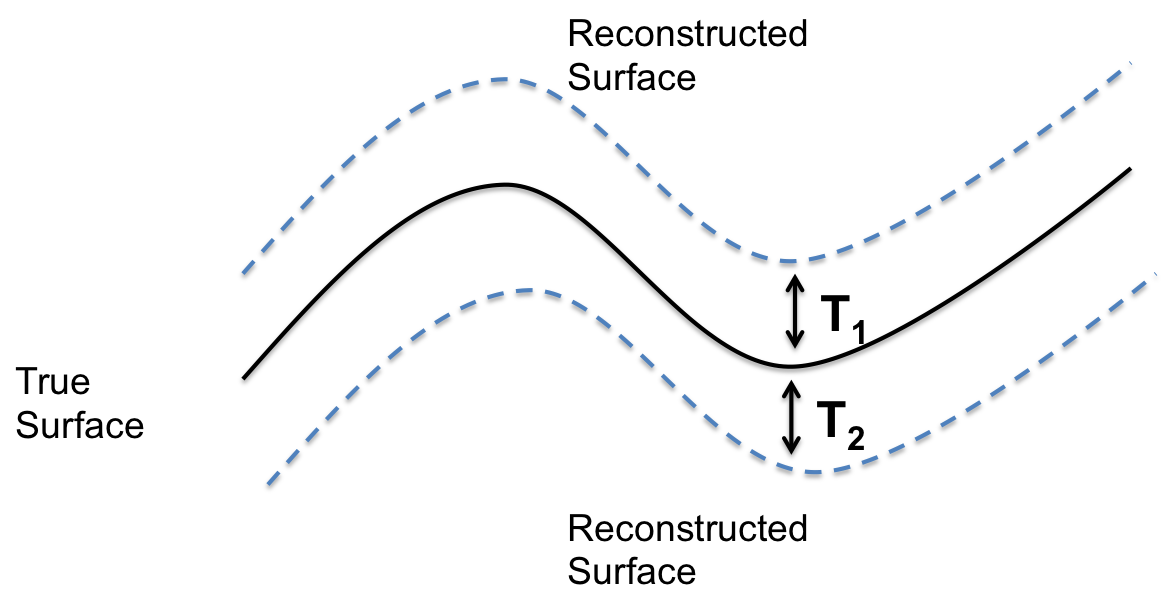
\includegraphics[scale=0.25]{deformation.png}
	\caption{Measured surfaces being deformed to the true surface.}
	\label{fig:deformationDiagram}
\end{figure}


\section{Volumetric Object Segmentation}
The final stage in the proposed object reconstruction pipeline is the segmentation of the object voxels from those that have had measurements fused 
from the background. This segmentation is formulated within a CRF framework, where each node in the CRF represents a set of neighbouring voxels in space, 
with connections being made between adjacent neighbourhoods. The process of segmentation can be posed as an energy minimisation problem over a cut in voxel space, 
such that a segmentation in 3D is obtained. The following energy function consists of the unary posterior probabilities over appearance accumulated during the fusion 
process for a region in space and an additional pairwise smoothing term representing the physical appearance similarity of the object region represented by the voxel 
neighbourhoods $\gamma$ and $\gamma^{'}$:
\begin{equation}
\begin{split}
E_{n} = \prod_{t=0}^{\infty} \prod_{\psi \in \Phi_{n}} P(\psi \in \Psi | \Omega_{t}, p_{t}) + P(\mathbb{E}[c]_{\gamma} | \mathbb{E}[c]_{\gamma^{'}})
\end{split}
\end{equation}
where $c$ represents the set of colour measurements fused in to the voxels within a given neighbourhood, for all $N$ subvolumes.

\section{Implementation Notes}
The probabilities that are accumulated into the volume are generated from a Random Forest based appearance model using patch based features encompassing 
appearance and surface information, such as depth gradients, initialised prior to reconstruction by a user interaction in the first frame. There are two 
classes in the appearance model, one for the foreground object and one for the background, with the foreground object indicated by a bounding box on the 
first RGB frame.

An overview of the processing pipeline for the proposed system is outlined in Figure \ref{pipelineDiagram}.
\begin{figure*}[!t]
	\centering
	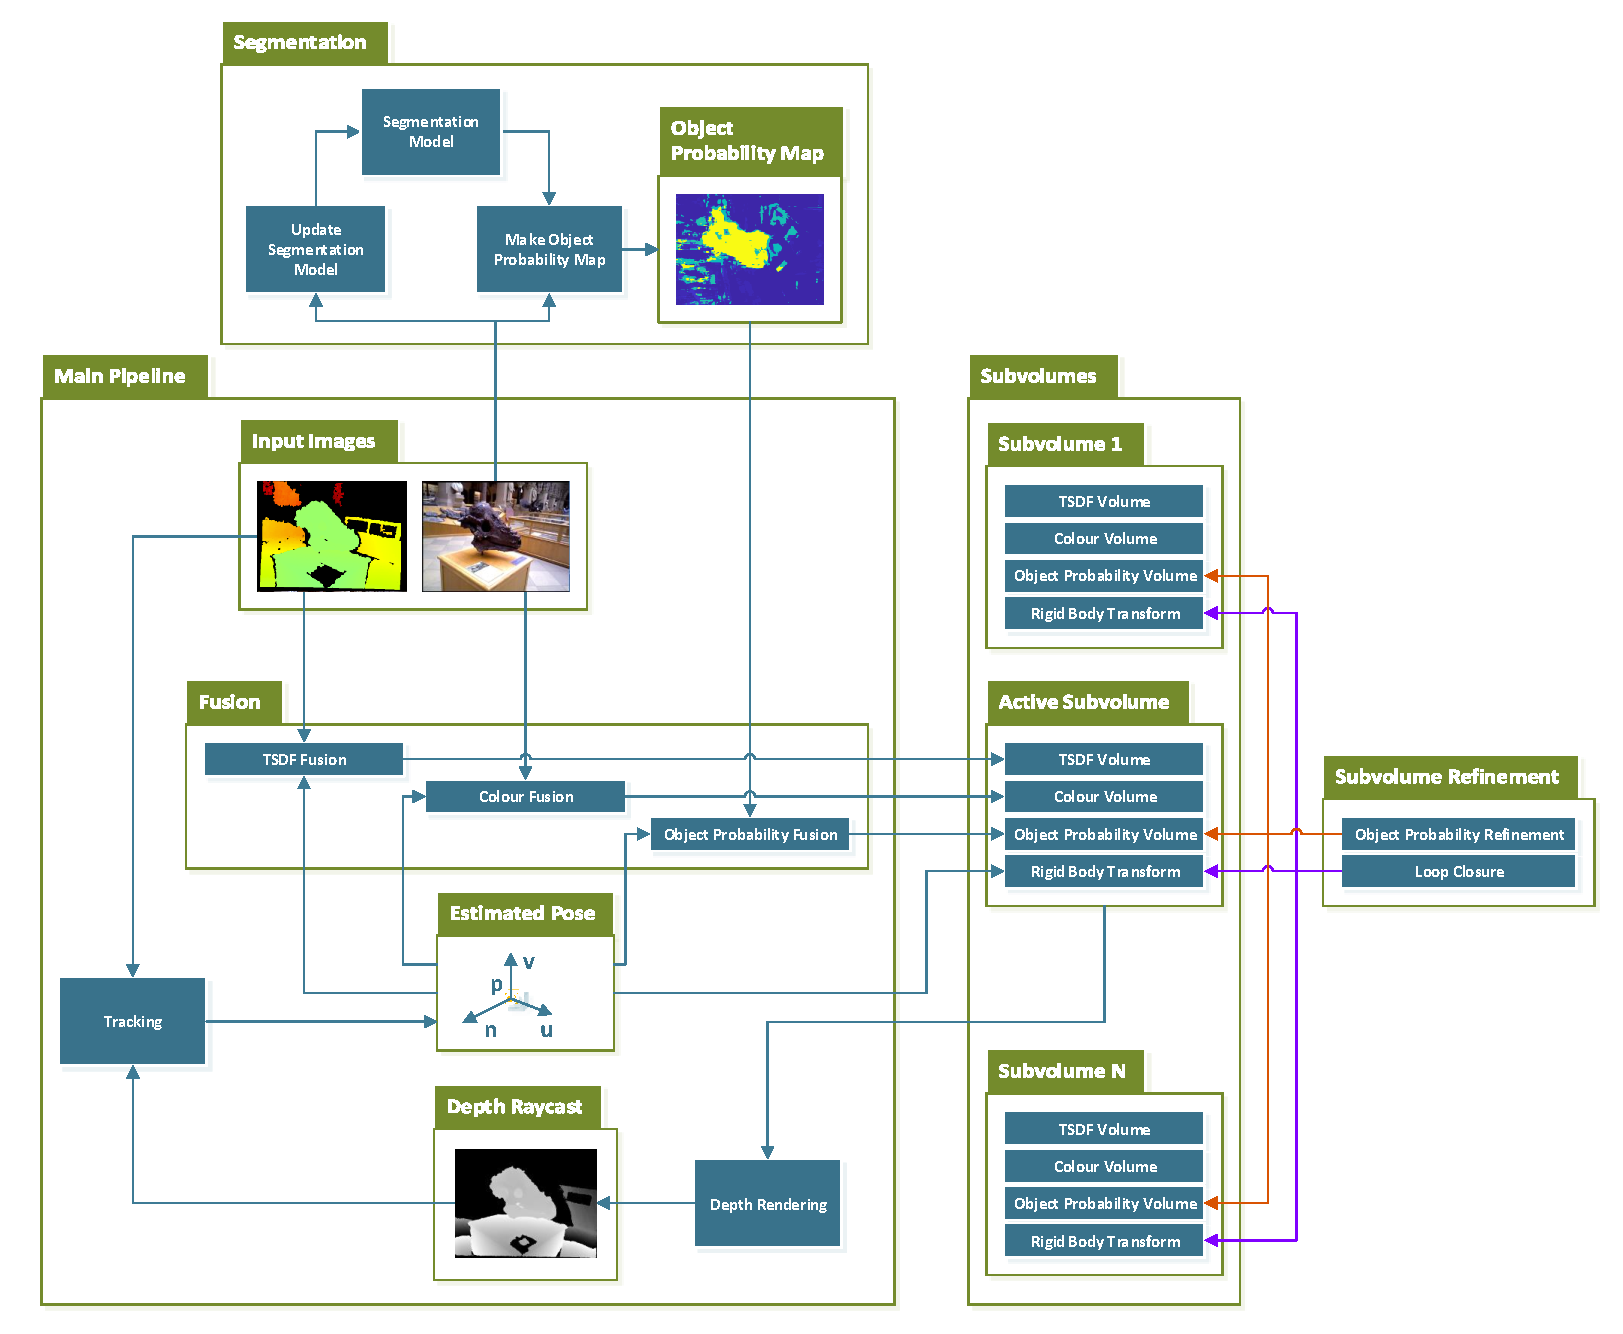
\includegraphics[scale=0.33]{pipeline.pdf}
	\caption{Object reconstruction pipeline.}
	\label{pipelineDiagram}
\end{figure*}

\section{Results}
To evaluate the performance of our system we perform experiments that draw comparisons in terms of quantitative pose estimation and qualitative reconstruction quality and efficacy.
Firstly, pose estimation is evaluated against a well established dense SLAM system \cite{Prisacariu2014}, with the primary difference being that in the benchmark system, the entire 
visible scene is used for pose estimation, whereas in our system only the object is tracked.
Qualitative comparisons are also drawn between the reconstructions of our system versus those of the system described in \cite{Ren2013}.

We evaluate the system on a set of objects of different sizes, some sequences with the object moving, others with the camera moving. However, it should be noted that in the case of the 
comparisons with the dense SLAM system it is not possible to evaluate the object motion sequences due to the tracking of the entire scene. Object motion with a static scene in this case 
would serve only to corrupt the scene model and tracking results, due to the systems inability to handle dynamic scenes.

\subsection{Pose Estimation Quality}
In this section we present quantitative results of our systems ability to maintain tracking robustness when tracking only an object and not the scene. In addition, the outputted trajectories 
of our system demonstrate less tracking drift and a robustness to loop closure events. We evaluate on <N> sequences of objects where the motion is restricted to camera only for the reason 
previously outlined. At this point it should be highlighted that the benchmark system has the advantage of an increased amount of geometry from which instantaneous poses can be estimated.
In the following experiments tracking is performed using only geometry cues from the rendered models and instantaneous depth frame.\\

Tracking between the two systems is evaluated w.r.t. ATE(Absolute Trajectory Error) as outlined in \cite{sturm12iros} and is summarised in Table \ref{ateTable}
\begin{table}[!t]
	{\small
		\begin{center}
			\begin{tabular}{l@{\hskip 1cm} c c}
				\emph{Sequence Name} & \emph{ATE}\\
				\midrule
				\textsf{Chair} & 0.048197\\
			\end{tabular}
		\end{center}
	}
	\caption{The absolute trajectory error (ATE) results (in metres, lower is better) achieved by our approach in comparison to the baseline InfiniTAM.}
	\label{ateTable}
\end{table}

\subsubsection{Chair Sequence}
In this sequence a static chair is reconstructed by moving the camera in an approximately circular fashion around with some repetitive camera motion at the end of the sequence to test 
the loop closure ability of the systems. The outputted trajectories may be found in Figure \ref{chairTrajectory}.
\begin{figure}[h]
	\centering
	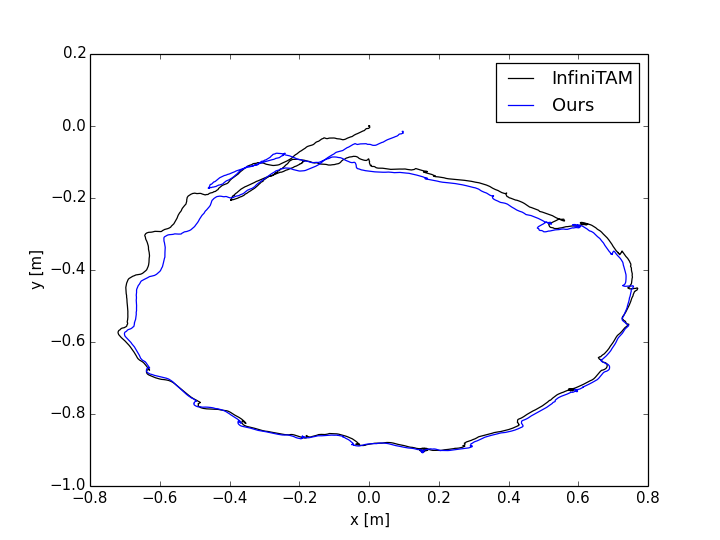
\includegraphics[scale=0.25]{plots/chairTrajectories.png}
	\caption{Trajectories outputted by the InfiniTAM dense SLAM system and our system.}
	\label{chairTrajectory}
\end{figure}
As can be seen in figure \ref{chairTrajectory} the robustness deficit when tracking with significantly is minimal, with the benchmark system appearing to incur cumulative tracking drift, as can be seen 
by the outwards `spiral' effect in the trajectory plots. In terms of overall ATE, the comparison between the two systems yields an ATE of \textbf{0.048197}.

\subsubsection{Cat Ornament Sequence}
%

\subsubsection{Teddy Sequence}

\section{Discussion}
As has been demonstrated in this paper, our system is efficacious in 3D object 
reconstruction. Our system is able to reconstruct closed object models on sequences for which an alternative, state of 
the art system \cite{Ren2013} fails to converge to any reasonable solution. In addition, we show robust odometry on an 
established SLAM benchmark, despite the difficulty of tracking only the objects surface vs the entire scene. Finally,
in spite of our use of ICP for pose estimation with ambiguities, our system is capable of robustly reconstructing a 
variety of objects.

{\small
\bibliographystyle{ieee}
\bibliography{bibliography}
}

\end{document}
